% Straight up stealing preamble from Eli Holmes 
%%%%%%%%%%%%%%%%%%%%%%%%%%%%%%%%%%%%%%START PREAMBLE THAT IS THE SAME FOR ALL EXAMPLES
\documentclass{article}

%Required: You must have these
\usepackage{Sweave}
\usepackage{graphicx}
\usepackage{tabularx}
\usepackage{hyperref}
\usepackage{natbib}
\usepackage{pdflscape}
\usepackage{array}
\usepackage{gensymb}
%\usepackage[backend=bibtex]{biblatex}
%Strongly recommended
 %put your figures in one place
 
%you'll want these for pretty captioning
\usepackage[small]{caption}

\setkeys{Gin}{width=0.8\textwidth} %make the figs 50 perc textwidth
\setlength{\captionmargin}{30pt}
\setlength{\abovecaptionskip}{0pt}
\setlength{\belowcaptionskip}{10pt}
% manual for caption http://www.dd.chalmers.se/latex/Docs/PDF/caption.pdf

%Optional: I like to muck with my margins and spacing in ways that LaTeX frowns on
%Here's how to do that
 \topmargin -2cm   
 \oddsidemargin -0.04cm  
 \evensidemargin -0.04cm % same as oddsidemargin but for left-hand pages
 \textwidth 16.59cm
 \textheight 22.94cm 
 %\pagestyle{empty}    % Uncomment if don't want page numbers
 \parskip 7.2pt      % sets spacing between paragraphs
 %\renewcommand{\baselinestretch}{1.5} 	% Uncomment for 1.5 spacing between lines
\parindent 0pt% sets leading space for paragraphs
\usepackage{setspace}
\usepackage{lineno}
\doublespacing
\usepackage{authblk}
%Optional: I like fancy headers
\usepackage{fancyhdr}
\pagestyle{fancy}
\fancyhead[LO]{Phenological sequences}
\fancyhead[RO]{2018}
%Does early phenology constrain later phenology?
%Early-season phenological events constrains late-season phenology.
%Early-season phenology constrains late-season phenology.
%Early-season life-events contrain late-season events.
%Timing is everything: Early-season phenology constrains late-season phenology
%The order of events: How early-season phenology shapes later-season phenology
%The shape of the season: How early-season phenological define events that follow
%How do previous phenological events constrain later events?
%How sequential phenological events determine the shape of a season
%sally likes"the shape of the season"
%%%%%%%%%%%%%%%%%%%%%%%%%%%%%%%%%%%%%%END PREAMBLE THAT IS THE SAME FOR ALL EXAMPLES
\linenumbers

%Start of the document
\begin{document}

% \SweaveOpts{concordance=TRUE}
\bibliographystyle{/Users/aileneettinger/citations/Bibtex/styles/amnat.bst}
\title{Phenological sequences: how early-season events define those that follow} %Other title ideas: 1. Phenological sequences: Early-season events affect later-season events; The shape of the season: how early phenological events define those that follow 
\author[1,2,a]{A. Ettinger}
\author[1]{S.Gee}
\author[1,3]{E.M. Wolkovich}
\author{A.K. Ettinger, S. Gee, and E.M. Wolkovich}
\affil[1]{Arnold Arboretum of Harvard University, Boston, Massachusetts 02131, USA}
\affil[2]{Tufts University, Medford, Massachusetts 02155, USA}
\affil[3]{Forest and Conservation Sciences, University of British Columbia, Vancouver, BC V6T 1Z4, Canada}
\affil[a]{Corresponding author; email: aettinger@fas.harvard.edu; phone: 781-296-4821; mailing address: 1300 Centre Street, Boston, Massachusetts 02140, USA }

%\date{\today}
\maketitle %put the fancy title on
%\tableofcontents   %add a table of contents
%\clearpage
%%%%%%%%%%%%%%%%%%%%%%%%%%%%%%%%%%%%%%%%%%%%%%%%%%%

%We will submit this paper as a ``brief communication' at American Journal of Botany (``short (3000-5000 word) research articles reporting exciting, significant new findings. They include no more than 4 figures and tables, combined. Manuscripts, and their abstracts, should be organized as described for Research articles.") or a ``rapid report" at New Phytologist.

\section*{Abstract}
\subsection*{Premise of the study}
Plant phenology is a critical trait as the timings of phenophases such as budburst, leafout, flowering, and fruiting, are important to plant fitness. Despite much study about when individual phenophases occur and how they may shift with climate change, little is known about how multiple phenophases relate to one another across an entire growing season. We test the extent to which early phenological stages constrain later ones, throughout a growing season across 25 angiosperm tree species. 
\subsection*{Methods}
We observed phenology (budburst, leafout, flowering, fruiting, and senescence) of 118 individual trees across 25 species, from April through December 2015. 
\subsection*{Key results}
%EMW: These sentences feel a little unrelated now and the results feels especially unrelated to the conclusions. Some edits below (including a sentence I have already commented out) but I think needs a little more help. 
We found that early phenological events weakly (most r\textsuperscript{2} < 0.30) constrain most later events, with the strongest constraints (maximum r\textsuperscript{2}= 0.43) seen between consecutive stages. In contrast interphase duration was a much stronger predictor of phenology (r\textsuperscript{2}=0.17-0.98), especially for reproductive events (r\textsuperscript{2} >0.7), suggesting that the development time of flowers and fruits constrain the phenology of these events.
\subsection*{Conclusions}
We found that much of the variation in later phenological events can be explained by the timing of earlier events and by interphase durations. This highlights that a shift in one phenophase may often have cascading effects on later phases, thus accurate forecasts of climate change impacts should include multiple phenophases within and across years. 

\section* {Key words}
plant phenology, climate change, budburst, leafout, flowering, fruiting, senescence, angiosperm, tree, arboretum
\section* {Introduction}
Plant phenology, the timing of recurring life-events such as leafout and flowering, is a critical trait that affects individual fitness, population abundance, agricultural and natural productivity, and global climate, through its role in carbon sequestration \citep{chuine2001,cleland2007,willis2010,miller-rushing2010,craine2012}. Advancement of budburst, leafout, and other phenophases are some of the most widely documented biological impacts of anthropogenic climate change, and phenology is likely to be further altered by future climate change \citep{parmesan2006}. Because of its important role in many ecosystem services and in the global climate cycle, improved understanding and forecasting of tree phenology would aid in planning and preparing for climate change impacts.

\par Despite the observation that spring phenology generally shifts earlier with warmer temperatures, dramatic variation exists in phenological responses to climate. Temperature is thought to be a major factor controlling phenology of temperate tree species \citep{parmesan2006,richardson2006,morin2010,schwartz2013,clark2014b}, but some populations and species have not shifted their phenology with recent warming \citep{wolkovich2012}. In addition, different tree species vary widely in the timing of leafout and other phenological processes, even when exposed to the same environmental conditions \citep{lechowicz1984,primack2009c}. Spring leafout, for instance, can span weeks among coexisting tree species \citep{lechowicz1984}. It has been proposed that, in addition to external environmental drivers such as temperature, some drivers of plant phenology are ``endogenous." That is, phenological sequences are affected by changes in internal tree functions that may not be related to climate or other environmental factors \citep{borchert1992,marco2002}. As an example, inflorescence architecture may affect the sequence of leafout to flowering in trees \citep{marco2002}. 

\par One important, but often neglected, feature of plant phenology is that events are sequential: leaf budburst comes before leafout, flowering comes before fruiting, and so on. This ordering is an endogenous factor that may constrain phenological responses to climate change. For example, if flowering requires a minimum development time following leafout (e.g. to acquire sufficient carbon), then flowering time may be constrained to shift no more than leafout timing has with recent climate change. This would be the case even if a greater advance in flowering may benefit the plant, for example if warmer springs have caused pollinator activity to shift earlier \citep{polgar2013, thackeray2010}

\par The extent of constraints between phenological events is unknown, however, because few studies have integrated across consecutive events throughout a growing season \citep{wolkovich2014}. Instead, researchers generally focus on one or two phenophases per study. Early season events (budburst and/or leafout) have been extensively studied, often using climate-controlled growth chambers \citep[e.g.,][]{basler2012,laube2014}. A separate group of studies, comprised of long-term observational data, focuses primarily on flowering only \citep[e.g.,] []{fitter2002,millerrushing2008}. Interest has recently surged in senescence, which had been less studied historically \citep {parmesan2006}, but many of these studies focus \textit{only} on senescence \citep[e.g.,][]{taylor2008,archetti2013,jeong2014}. A contemporary meta-analysis highlights the lack of data on multiple phenophases: only five out of 51 phenology studies (9.8\%) included data on both leaf and flower phenology \citep{wolkovich2012}. 

\par When research has looked across stages, important links have often been found. For example, later leafing in a given year may be associated with later flowering, and fall senescence has been associated with both fruit maturation and spring phenology, in different studies \citep{lechowicz1995,keenan2015,liu2016}. In contrast, other research that has quantified multiple phenological events over time has documented that some phenophases may shift asynchronously with climate change \citep[e.g., spring events are occurring earlier as fall events have gotten later, first-flower dates have shifted earlier whereas last-flower dates have not,][]{menzel2006,caradonna2014}. These insights and complications demonstrate the need to better understand how phenological stages relate to one another across an entire growing season \citep{wolkovich2014}.

\par Here, we examine the extent to which early-season phenological events constrain later events across tree species planted in the same environment. Specifically, we test two hypotheses:
\begin{itemize}
\item \textit{Hypothesis 1: Previous phenological events constrain later events;} e.g., late-fruiting species set fruit late in the season, because they flower and leafout late (Figure \ref{fig:hyp}). To be consistent with this hypothesis, we expected earlier events, such as flowering, would predict later events, such as fruiting. If constraints are strong, then, across all species, we expected that previous events should predict later events with a slope of one, indicating that the later event happens a set number of days (represented by the intercept) after the previous event (Figure \ref{fig:hyp}). If constraints are weak, we expected to find relationships between later and earlier events, though the slope may be less than one. No relationship would suggest that earlier events do not constrain later events.

\item \textit{Hypothesis 2: Interphase duration constrains phenology;} e.g., late-fruiting species set fruit late in the season because they require longer maturation time (Figure \ref{fig:hyp}). To be consistent with this hypothesis, we expected that the interphase duration (the number of days between two phenological events) between earlier and later events would be a strong predictor (e.g., a large r\textsuperscript{2}) of the later event, regardless of the timing of the earlier event (Figure \ref{fig:hyp}). 
\end{itemize}
Testing these hypotheses addresses basic, critical questions about drivers of variation in temperate tree phenology. These questions remain unanswered despite decades of phenology research because previous field studies rarely (if ever) examined multiple phenophases spanning the entire growing season across a large number of tree species. 
\section* {Materials and Methods}
\subsection*{Study site and focal species}
This study was conducted at the Arnold Arboretum of Harvard University, a 281-acre park in Boston, Massachusetts, established in 1872. It contains a living collection of 3,825 woody plant taxa that are native to North America, Europe, and Asia. Arboreta are excellent resources for phenological studies across many species \citep [e.g., ][]{primack2009a}, particularly in temperate areas, since they may contain a higher diversity of tree species growing in one location than nearby natural areas. In addition, there is often high variation in phenology of species planted in arboreta, for public enjoyment of foliage and flowers throughout the season. For this study, we selected 25 focal angiosperm species with diverse flowering times, in order to maximize variation in phenology (Table 1). We selected up to five individuals of each species for the study, yielding a total of 118 individuals.

\subsection*{Phenology data collection}
We visited each individual once every 6-10 days throughout the growing season. Phenology observations in the spring began on April 6, 2015 (prior to any budburst occurring) and fall phenology observations ended on December 2, 2015 (at which point more than 95\% of leaves on all trees had changed color and dropped). We observed five phenological stages, which were quantified following the National Phenology Network (NPN) protocols \citep[for a full description see][]{denny2014}. The budburst phase was characterized by green leaf tips being visible at the tips of buds, and the leafout phase was characterized by visible fully unfolded leaves and petioles that had completely emerged from the buds. The flowering phase was when open flowers were visible, and the fruiting phase was defined by ripe fruit being visible. Leaf senescence was characterized by leaves changing from green to fall colors. On each observation day, we estimated the presence and abundance of each phenophase on each individual tree.
\par From the field observation data, we extracted the day-of-year (DOY) of the first observed occurrence of a given phenological phase. Budburst and fruiting DOY were defined as the first day when three or more burst leaf buds or ripe fruits, respectively, were observed on the individual. Leafout, flowering, and leaf senescence DOY were defined as the first day when 5\% or more of the individual was leafing out, flowering, or showed fall colors, respectively \citep{denny2014}. 
From these individual tree phenology observations, we calculated species-level mean start dates and for all phenophases, for use in our statistical analyses. We used these mean start dates to calculate interphase durations between phenophases. 
\subsection*{Statistical analyses}
To understand the extent to which previous phenological events constrain later events across species (Hypothesis 1, Figure \ref{fig:hyp}), we fit linear models in which the response variable was phenological stage (i.e., the species' mean DOY of leafout, flowering, fruiting, or senescence), and the predictor was previous phenological stage. Thus, budburst was excluded as a response variable, because it was the earliest stage we quantified, and senescence was excluded as a predictor variable because it was the latest stage we quantified. We therefore fit 10 separate regression models, estimating the intercept of the relationship between later and previous phenological phases, and forcing the slope to be one (Hypothesis 1, Figure \ref{fig:hyp}). In addition, we fit 10 models, with the same predictor and response variables, in which we estimated the best-fit slope and intercept (via least-squares, e.g., a standard regression model). Under Hypothesis 1, with strong constraints, we expected that the models with forced slopes should provide similar fit to the data as the standard regression models that estimate both slopes and intercepts. We compared fit of these two model structures using r-squared values, as well as Akaike's Information Criterion (AIC). 
\par To understand the extent to which interphase duration constrains later phenological events (Hypothesis 2, Figure \ref{fig:hyp}), we fit linear models in which the response variable was phenological stage, and the predictor was the number of days between phenological stages. Thus, as above, budburst was excluded as a response variable. We therefore fit 10 different models, each with one of four phenological stages as the response variable and one of the four interphase durations as a predictor. To investigate the effect of interphase duration, separate from the constraint imposed by the inherent ordering of events, we fit models in which the interphase durations were randomized with respect to the timing of the earlier phenophase across species. We did this resampling of interphase duration 999 times for each model structure. If our expectation of later events being constrained by interphase duration was supported, then the best-fit slope should fall within the resampled models' slope estimates. Furthermore, if the constraints imposed by interphase duration were due primarily to the inherent ordering of events, then the randomized models should include a narrow range of possible slopes. To examine these possibilities, we compared the range of slopes of all the resampled models to the slope of the fitted model. 
\par All analyses were conducted in R version 3.2.4 \citep{rcoreteam2017}, and code is available in the Supplemental Materials.

\section* {Results}
\par We monitored five phenophases, which varied in duration. First budburst date occurred over 32 days and first leafout date occurred over 30 days in the spring, across all focal individuals (Figure S1) and species (Figure \ref{fig:focsp}). Flowering phenology occurred over a longer period than budburst and leafout, spanning 131 days from late April to September. The first observation of ripe fruit spanned 175 days, and the start of leaf senescence occurred over 56 days across all individuals and species. Most species (20/25) spent the majority of the growing season in the reproductive phenological phases (i.e., flowering and fruit development), and most species (23/25) began leaf budburst prior to flowering, though leaf development overlapped with flowering in some species (Figure \ref{fig:focsp}). The majority of species (15/25) produced ripe fruit prior to beginning senescence (Figure \ref{fig:focsp}).

\par We found that the timing of early phenological stages predicted the timing of later stages in many cases (Figures \ref{fig:focsp}-\ref{fig:latevearly}, Table S1). The strongest relationships (i.e., with the most variation explained) occurred between adjacent stages (those along the diagonal in Figure \ref{fig:latevearly}, such as leafout and budburst, fruiting and flowering). Even for adjacent phases, however, neither the forced slope models nor the regression models explained a large proportion of the variation in phenology (r\textsuperscript{2} < 0.30, in most cases). For three relationships (flowering versus budburst, flowering versus leafout, and fruiting versus flowering), the model fits were consistent with the constraint hypothesis---the forced slope model provided similar fit to the regression models and both models explained a significant amount of variation in phenology (Figure \ref{fig:latevearly}, Table S1). For four relationships, standard regression models explained much more variation than the forced slope models.   For two of these relationships(leafout versus budburst, and senescence versus fruiting), the regression models had slopes that were less than one and for the other two relationships (fruiting versus budburst and fruiting versus leafout), the regression models had slopes that were greater than one (Figure \ref{fig:latevearly}, Table S1).

\par We observed strong relationships (r\textsuperscript{2}>0.7) between phenology and interphase duration for the two reproductive phenophases (flowering and fruiting time, Figure \ref{fig:inter}, Table S2). Flowering DOY was strongly predicted by days between flowering and leafout (r\textsuperscript{2}=0.93), as well as by days between flowering and budburst (r\textsuperscript{2}=0.87). Fruiting DOY was strongly predicted by days between fruiting and flowering stages (r\textsuperscript{2}=0.74), by days between fruiting and leafout (r\textsuperscript{2}=0.98), and by days between fruiting and budburst (r\textsuperscript{2}=0.97). Senescence was predicted by days between senescence and budburst (r\textsuperscript{2}=0.74), days between senescence and leafout (r\textsuperscript{2}=0.82), and days between senescence and flowering (r\textsuperscript{2}=0.17); senescence was not affected by days between senescence and fruiting.  Leafout was not predicted by interphase duration (i.e., time since budburst). In all cases where later events were well predicted (r\textsuperscript{2}$>$0.7) by interphase duration, the best fit model was predicted by our null model (i.e., the randomizations).  However, the relationship between senescence and days between senescence and flowering was weaker than expected by our null model (see resampling estimates in Figure \ref{fig:inter},Table S2).

\section* {Discussion}
%EMW: edits below. 
\par The ordering inherent in phenology means most phenological stages are dependent---in some way---on those stages before: dormancy must be broken before buds can burst and flowers must be produced before fruit. Here we show how the major phenological stages of temperate trees are constrained by one or more earlier phenological stages. 

%EMW: Check spelling below and in document. 
\par All phenological stages we observed support Hypothesis 1: timing appears to be constrained by at least one previous phenological stage. Our findings are consistent with recent work suggesting that senescence time can be affected by earlier phenophases \citep{keenan2015,liu2016}, and suggest that this one relationship is part of larger suite of correlated phenophases. Consecutive events were correlated across both growth and reproductive phenophases (i.e., flowering and leafout were correlated to a similar degree as fruiting and flowering, Figure \ref{fig:latevearly}). These associations may occur because of endogenous dependencies between the two phases, because of a shared external driver such as growing degree days, or a combination of endogenous and external factors \citep{lechowicz1995}. Thus, environmental conditions in the winter or spring that may directly affect only early phenological stages, such as budburst, are likely to have cascading effects on later stages such as leafout, flowering, and fruiting. Our data suggest that, for most events, these effects are more apparent for consecutive stages (i.e., those along the diagonal in Figure \ref{fig:latevearly}), and are well-approximated by the forced slope model in some cases (Figure \ref{fig:latevearly}).

\par Although some of the variation in reproductive phenology (flowering and fruiting) was explained by previous phenology (Hypothesis 1), much more variation was explained by interphase duration (Hypothesis 2). Later flowering species generally required more time between flowering and leafout. Similarly, late fruiting species had longer interphase durations between the first observation of ripe fruit and first flowering date. It may be that late fruiting species require longer fruit development times to produce larger fruits or more highly-provisioned seeds. This would be consistent with previous theories that trees investing more resources into their offspring (i.e., having larger seeds) require more time to build resources \citep{bolmgren2008,sun2011}. There were notable exceptions to this general relationship, however. Some species set fruit later than expected, given their interphase duration between flowering and fruiting (\textit{Catalpa speciosa, Tilia americana, T. japonica}, Figure \ref{fig:inter}). These species also flowered later than expected, given their leafout DOY (Figure \ref{fig:latevearly}). External factors related to their ecology may be the cause; for example, these species are all insect-pollinated, so the timing of their pollinator activity may have affected their floral phenology \citep{elzinga2007}. %EMW: Are they the only insect-pollinated species? If not I am not sure how well this argument works (maybe move to results?). Also, I think the two responses you mentioned are related: to have set fruit later than expected based on interphase duration suggests that they flowered later ... no?

%EMW: Edits below, see what you think. It still needs some work to shorten and clarify ... if you see any options!
\par Despite our expectation of strong relationships between later phenophases and interphase durations (Figure \ref{fig:inter}), our results show two relationships that are weaker than expected. Leafout was not predicted by the interphase duration between budburst and leafout, and senescence was not predicted by the interphase duration between fruiting and senescence (Figure \ref{fig:inter}). We had expected that these two sets of phases would demonstrate \textit{stronger} constraints of interphase duration because they occur at the beginning and end of a bounded growing season \citep{letten2013}. The weak ability of interphase duration to predict leafout may be due to the distinct weather patterns in 2015 and how they interacted with species' cues for spring phenology. Trees have species-specific chilling and forcing requirements that must be met prior to leafing out, and are generally understood to be related to accumulations of warm and cold temperatures \citep[e.g.,][]{schwartz2010,chuine2010,clark2014b}. Because of this, the pattern of how quickly cooler and warmer temperatures accumulate across a growing season can impact how variable leafout is across species. In contrast to some years that have high variation in leafout date across species \citep{lechowicz1995}, in our study year (2015) many species leafed out close to DOY 130 (10 May), regardless of leafout-budburst interphase duration (which ranged from 0 to 20 days, Figure \ref{fig:inter}). This could be due to the temperature conditions particular to 2015: temperatures were colder than average in January through March, and then switched to above-average in late April and early May (www.bluehill.org). Such long periods of cold followed by rapid warming may have meant that chilling requirements were met for all species well before warm temperatures began, and then forcing requirements were rapidly met for many species (even if they had diverse requirements) leading to a flush of leafout in early May, across diverse species. Variation in the environment each year may alter how later phenophases are constrained by earlier events and highlights the need to better understand how such constraints vary across years and what underlies the remaining variation not explained by earlier phenophases.

%EMW: I made some edits but got a bit stuck... I wonder again if this species example could just move up to the results and the topic sentence (and paragraph) could become more: Variation in the environment each year may alter how later phenophases are constrained by earlier events and highlights the need to better understand how such constraints vary across years and what underlies the remaining variation not explained by earlier phenophases. OR Variation in the environment each year may alter how later phenophases are constrained by earlier events and highlights the need to better understand how such constraints vary across years and connect such variation to the large literature of what proximate cues trigger phenology. (This latter option would flow nicely into your next paragraph). 
\par Our results indicate that \textit{both} Hypothesis 1 and Hypothesis 2 are operating and can explain a substantial amount of the variation observed among species in a single year. For example although later fruiting is generally associated with later flowering (Figure \ref{fig:latevearly}), some species, such as \textit{Quercus alba} and \textit{Quercus grandifolia}, flower relatively early and fruit late; later fruiting for these species is instead associated with longer interphase duration between fruiting and flowering (Figure \ref{fig:inter}).  Understanding drivers of variation in phenological responses among species requires disentangling the ways that earlier phenology and interphase duration interact with one another, and with environmental conditions. Experimental manipulations will be beneficial for discerning the physiological and genetic bases for the relationships we observe \citep{flint1974}.

\par Our findings have important implications for improved forecasting of climate change induced shifts in phenology. A shift in one phase may have cascading effects on later phases, since each phase is linked to phases that occur before and after it \citep{wolkovich2014b}. Phenology models covering the whole annual cycle are rare for wild plants \citep[but see][]{chuine2001} and have not been used to forecast phenology at the community level. Our results highlight a clear need to conduct future multi-species phenology studies across entire growing seasons \citep{wolkovich2014}, and begs the question of how phenophases may be linked across years, as well \citep[e.g.,][]{elmendorf2016}. For example, the timing of spring budburst in one year may be related to the timing of budset the previous fall \citep {mimura2010}. Although relationships between phenophases have not been widely studied, there is a growing ecological literature on the concept of ``ecological memory," or the capacity of past states to influence present or future responses \citep {ogle2015}. The ecological memory of phenology has not been quantified, but may be critical for accurate forecasting, particularly for species like \emph{Quercus rubra}, which require more than one year for fruit maturation. Given the species-specific nature of phenological constraints, accurate forecasts of community-wide phenological shifts are likely to require species-specific information, such as fruit development time for fruiting forecasts, in addition to climate data \citep{diez2012}.

\section* {Conclusions}
We have shown that early and late phenological stages are strongly linked across the growing season, providing a new approach to explain some of the dramatic variation in phenological responses observed to date. Many studies have sought to identify the particular environmental drivers of phenology \citep [e.g.,][]{morin2010,schwartz2013}. Our findings here suggest that timing and duration of previous phenological states should also be examined. In addition, identifying the appropriate temporal window for both environmental and endogenous drivers is essential \citep{teller2016}. Because earlier phenophases define those that follow, the relevant time period for these drivers may extend further back in time than the single growing season we evaluated here. Multi-year studies will be critical to evaluate the extent to which phenological patterns are consistent among years that may vary in climate, as well as biotic conditions \citep [i.e., pollinator or pest populations,][]{lechowicz1995}. %Additional variation in phenological responses may be understood by incorporating phylogenetic approaches, and by exploring patterns at the individual, rather than species, level. 
A fuller understanding of phenological constraints and drivers of phenological variation offers the potential for improved forecasts of phenological shifts with climate change to help predict how ecosystem functions will be altered in the future. 

\section*{Acknowledgements}
The authors thank J. Davies, H. Eyster, D. Flynn, E. Forrestel, S. Golumbeanu, W. Friedman, R. Mcnellis, J. Samaha, J. Savage, and T. Savas for field and laboratory assistance and advice. We thank the curatorial, horticultural, and research staff of the Arnold Arboretum who made this work possible. Research was supported by the Harvard College Research Program (to S.G.), the Grants-In-Aid of Undergraduate Research program of the Museum of Comparative Zoology, the Harvard University Herbaria, and the Arnold Arboretum of Harvard University (to S.G.), and the National Science Foundation (NSF DBI 14-01854 to A.E.). Any opinion, findings, and conclusions or recommendations expressed in this material are those of the authors and do not necessarily reflect the views of the National Science Foundation.

\section*{Data Accessibility}
The data set for this study is available online at Knowledge Network for Biocomplexity \citep{gee2017}. 

\section*{Author contributions} All authors conceived of and designed the study and edited the manuscript; S.G. conducted the fieldwork; S.G. and A.E. analyzed the data and wrote the manuscript.

\bibliography{/Users/aileneettinger/citations/Bibtex/mylibrary}

\section* {Tables}

\begin{table}[p]
 \caption{\textbf{Study species.} Twenty-five angiosperm species were selected based on their flowering phenology in long-term records of the Arnold Arboretum. The flowering patterns we observed during our one year of data collection did not always perfectly match these long-term patterns. The number of individuals of each species observed at the Arnold Arboretum from spring through fall 2015 is in parentheses.}
\begin{footnotesize} 
  \begin{tabular}{| p{5.5cm} | p{5.5cm} | p{5.5cm} |}
  \hline
 \bf{Early-season flowering} & \bf{Mid-season flowering} & \bf{Late-season flowering} \\ \hline
  \textit{Aesculus flava} (5) & \textit{Carya glabra} (5) & \textit{Catalpa speciosa} (5) \\ 
  \textit{Betula alleghaniensis} (5) & \textit{Carya ovata} (5) & \textit{Kalopanax septemlobus} (3) \\ 
  \textit{Betula nigra} (5) & \textit{Crataegus crus-galli} (5) & \textit{Styphnolobium japonicum} (5) \\ 
\textit{Gleditsia triancanthos} (5) & \textit{Fagus engleriana} (4) & \textit{Tilia americana} (5) \\ 
\textit{Liriodendron tulipifera} (5) & \textit{Fagus grandifolia} (5) & \textit{Tilia japonica} (5) \\ 
\textit{Phellodendron amurense} var. \textit{lavallei} (4) & \textit{Fraxinus chinensis} (5) &\\ \textit{Populus deltoides} ssp. \textit{deltoides} (5) & \textit{Liquidambar styraciflua} (5) & \\ 
\textit{Pyrus calleryana} var. \textit{dimorphophylla} (3) & \textit{Platanus occidentalis} (5) & \\ 
\textit{Pyrus ussuriensis} var. \textit{hondoensis} (5) & \textit{Quercus glandulifera} (4) & \\ \textit{Quercus alba} (5) & \textit{Quercus rubra} (5) & \\ \hline
   \end{tabular}  
\end{footnotesize} 
  \end{table}
\clearpage

\section* {Figures}
\begin{figure}[p]
 \centering
 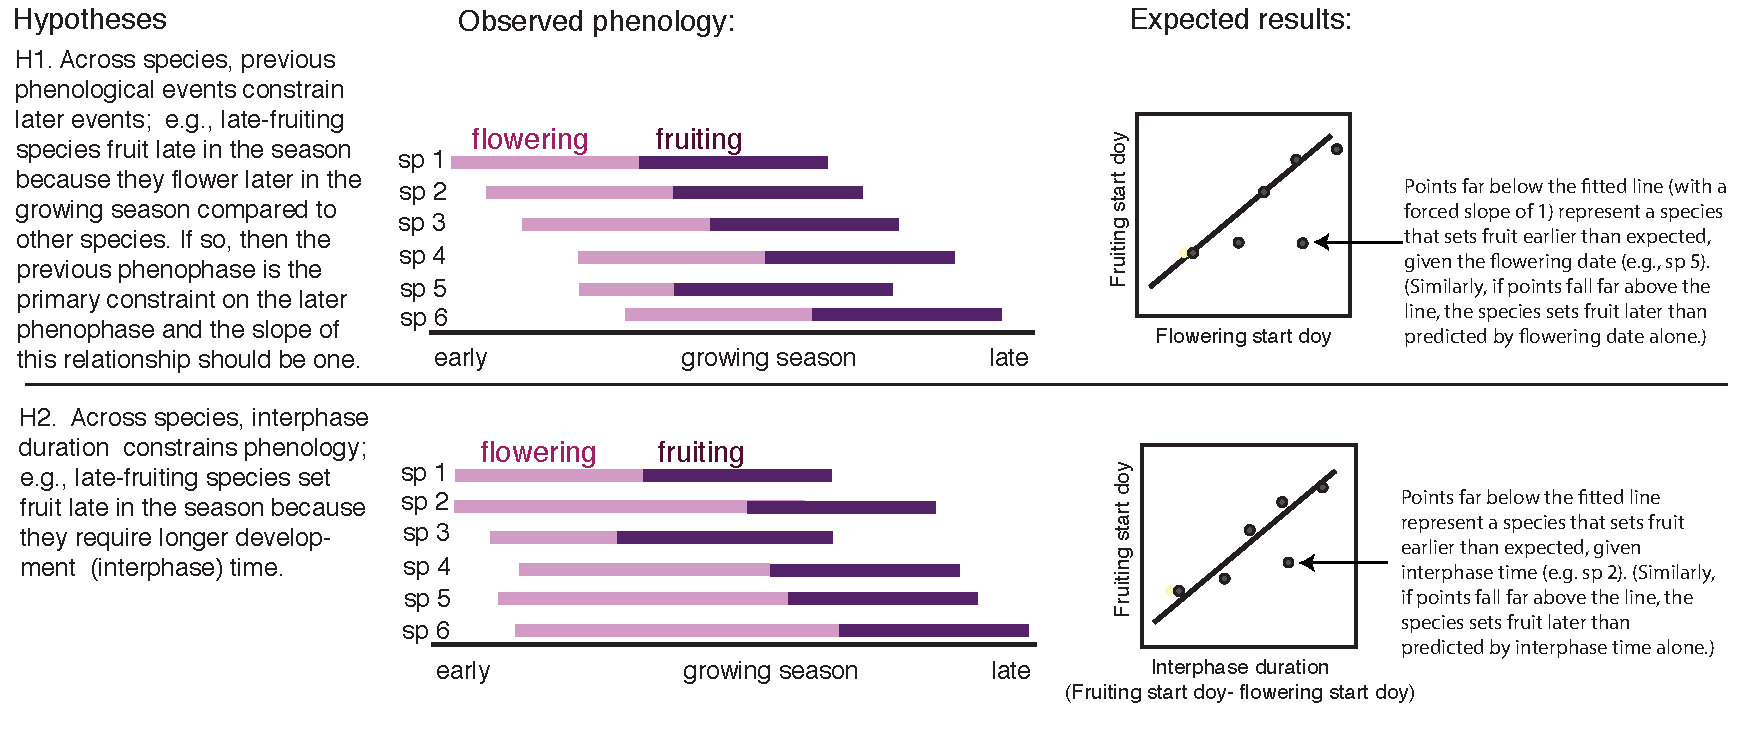
\includegraphics{../analyses/figures/hypotheses3.pdf} 
  
 \caption{\textbf{Hypotheses.} We show flowering and fruiting as examples of consecutive phenological events. We expected the same patterns for other consecutive events, such as leaf budburst and leafout. Interphase duration is the time between phenological events, e.g., the number of days between the first day of flowering and the first day that ripe fruit were observed.} 
 \label{fig:hyp}
\end{figure}
 
\begin{figure}[h]
 \centering
 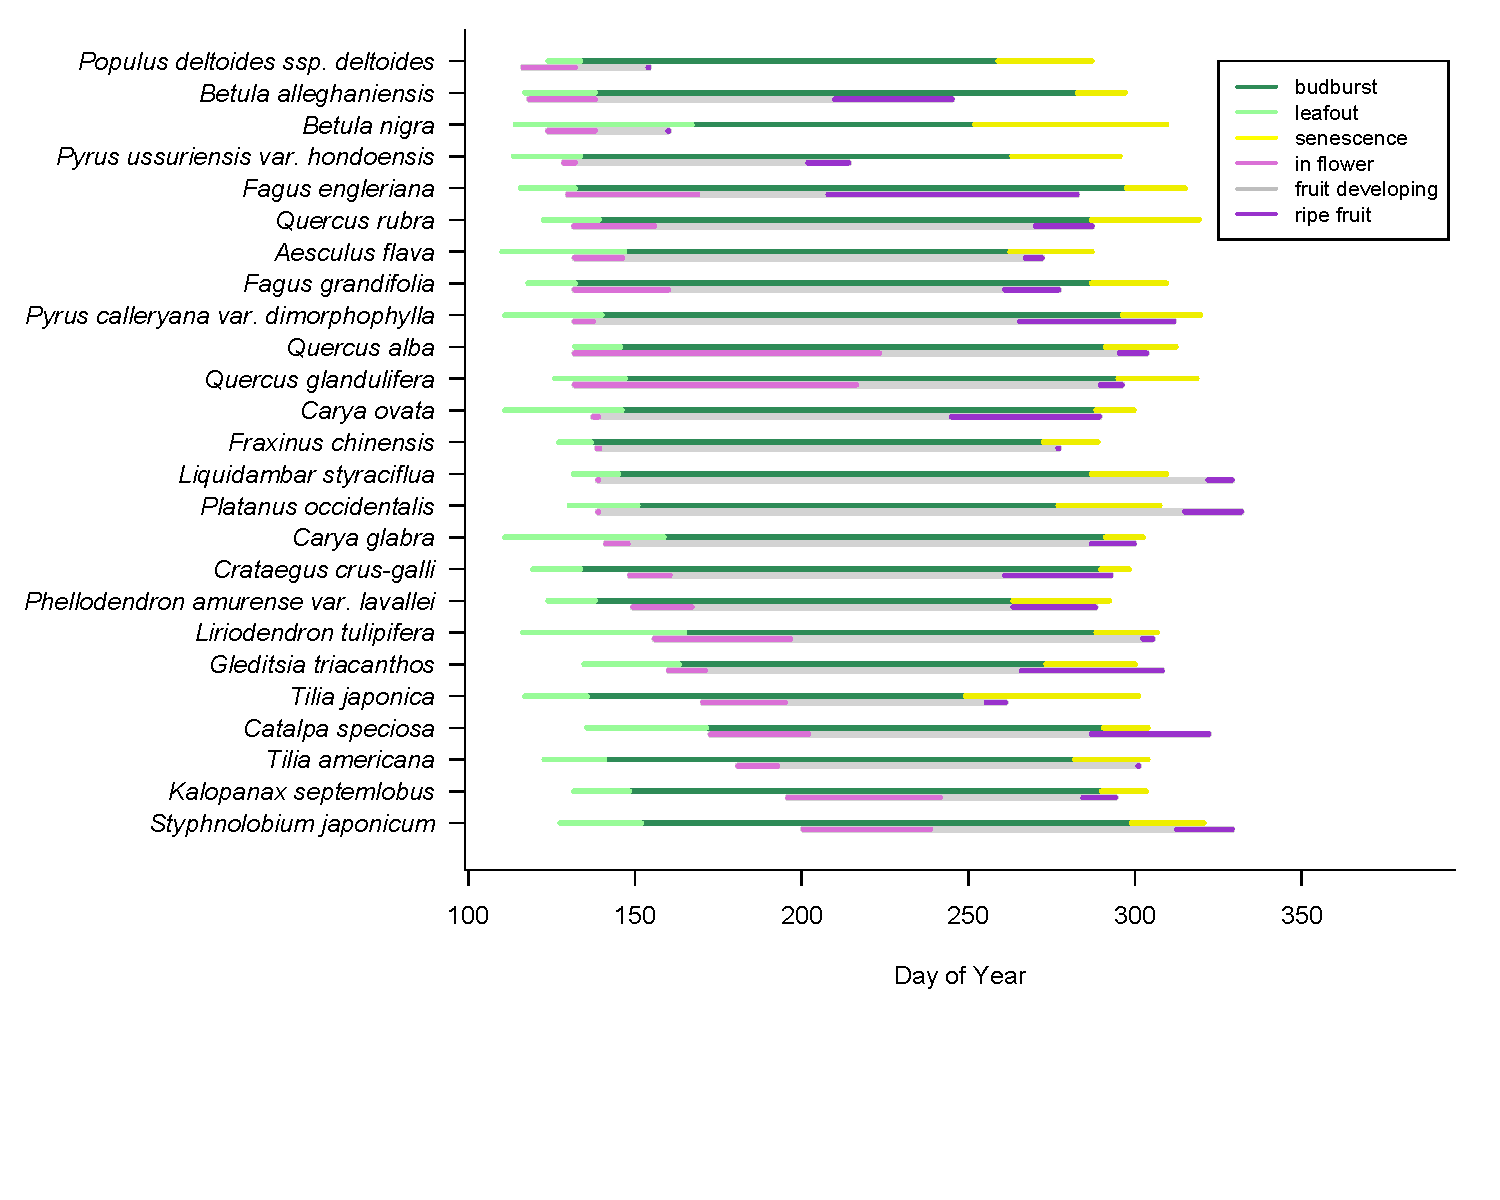
\includegraphics{../analyses/figures/grosea_repsort_ripefruit_legend.pdf}
 \caption{\textbf{Species' phenology during the 2015 growing season, ordered by mean first-flower dates.} Growth phenology is shown for budburst (from its mean start day-of-year to the mean start day-of-year for leafout, across all individuals within a species), leafout (from the mean day-of-year when fully-expanded leaves were first observed through the start of senescence), and senescence (from the mean day-of-year when leaves first began changing color through the mean day-of-year when more than 95\% of leaves on the tree had changed color). Reproductive phenology is shown for flowering (from the mean day-of-year when flowers first appeared to the mean day-of-year when fruits first appeared, across all individuals within a species) and fruiting (from the mean day-of-year when fruits first appeared to the mean day-of-year when more than 95\% of fruits were first observed as ripe).}
 \label{fig:focsp}
\end{figure}
 
 \begin{figure}[h]
 \centering
 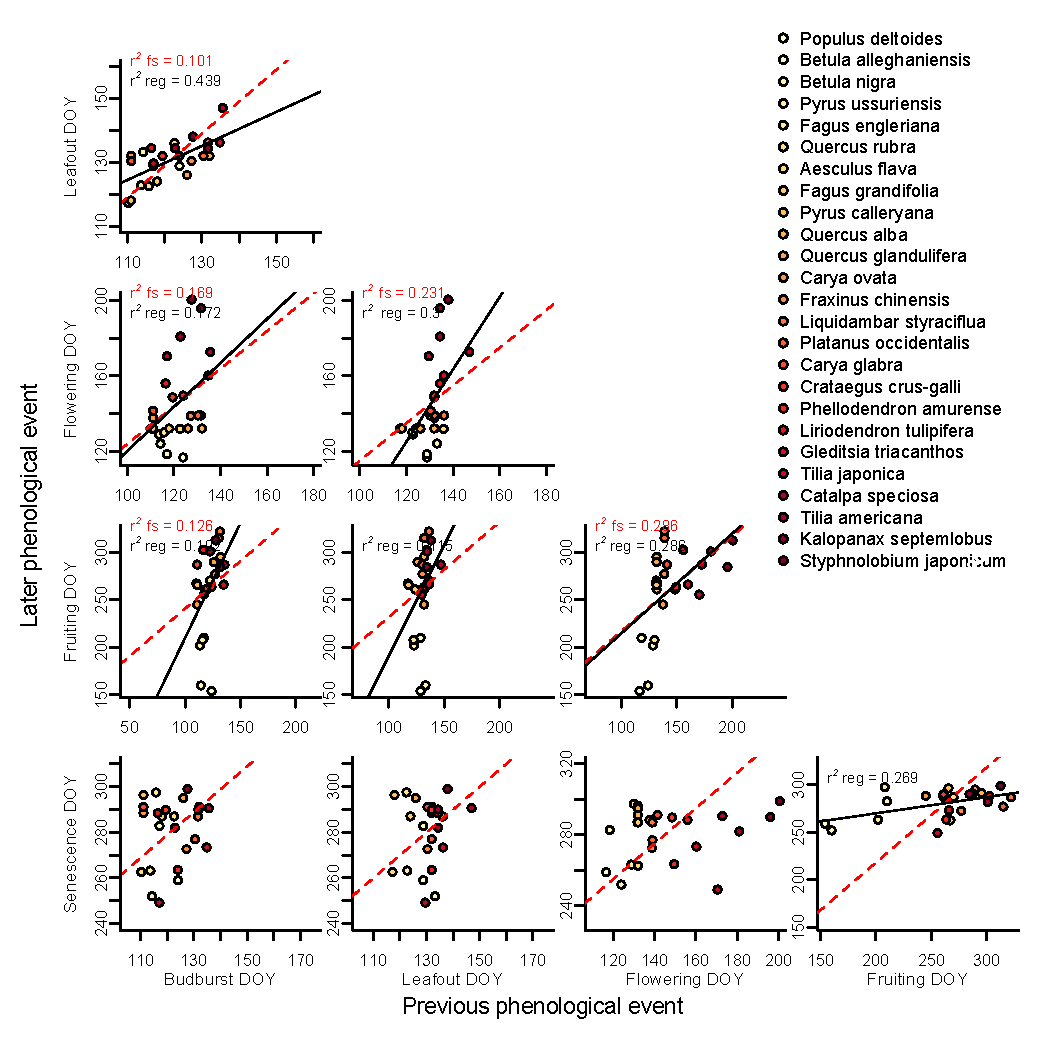
\includegraphics{../analyses/figures/Hyp1_forcedslope_samerange.pdf}
 \caption{\textbf{Relationships among phenological stages across the 25 focal species.} Linear models were fit with the species-level mean day-of-year (DOY) of the later phenological stages as the response variable, and mean day-of-year of earlier stage as the explanatory variable. Models with a forced slope of 1 are shown by dashed red lines, and r\textsuperscript{2} is given when r\textsuperscript{2}>0.10. (``fs", in red). r\textsuperscript{2} for standard regression (``reg," in black) and lines for these models are shown when r\textsuperscript{2}>0.10 (solid black lines). Full model statistics are summarized in Table S1 in the Supplemental Materials. Species in the legend are ordered from early to late first-flower dates.} 
 \label{fig:latevearly}
\end{figure}
\begin{figure}[h]
 \centering
 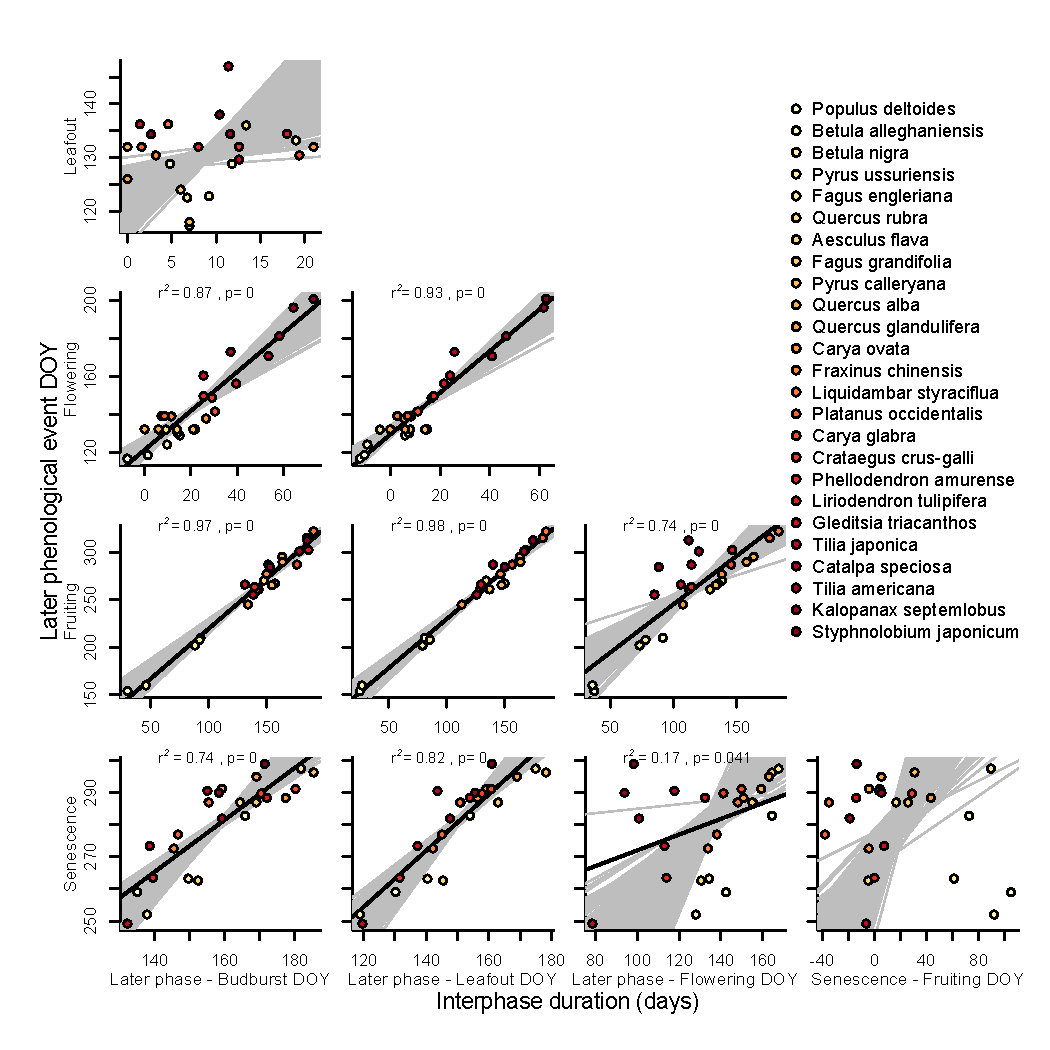
\includegraphics{../analyses/figures/Hyp2.pdf}
 \caption{\textbf{Relationships among phenological stages and interphase duration across the 25 focal species.} Interphase duration (x-axis) is the time between the start of the earlier phenological event and the start of the later phenological event (e.g., the number of days between the species' mean start of flowering and its mean start of fruiting). Linear models were fit with the species-level mean day-of-year (DOY) of the later phenological stages as the response variable, and interphase duration as the explanatory variable. Solid lines (representing model fit) and r\textsuperscript{2} are shown when r\textsuperscript{2}>0.10. Gray lines represent model fits when interphase was randomized with respect to the timing of the earlier phenophase (in some cases the range of possible relationships is quite narrow, given the constraints of ordering inherent in phenological events). When our null expectation of later events being constrained by interphase duration was supported, the best-fit slope (black line) will fall within the randomized lines (in gray). Full model statistics are summarized in Table S2 in the Supplemental Materials. Species in the legend are ordered from early to late first-flower dates.}
  \label{fig:inter}
  \end{figure}

%%%%%%%%%%%%%%%%%%%%%%%%%%%%%%%%%%%%%%%%
\end{document}
%%%%%%%%%%%%%%%%%%%%%%%%%%%%%%%%%%%%%%%%
